\chapter{Map of Profiles} % Main chapter title

\label{Chapter6} % Change X to a consecutive number; for referencing this chapter elsewhere, use \ref{ChapterX}

Load profiles can be grouped and sorted into various ways and forms.
Main attributes in order for profiles to be mapped are: 

\begin{outline}

\1 Way of metering or presenting a profile
\2 Main meter metering
\2 Appliance level metering

\1 By time range of profile 
\2 Daily
\2 Weekly
\2 Monthly
\2 Yearly

\1 Way of measuring usage
\2 Average power use 
\2 Activation or frequency of activation
\2 other (On time distribution, or on time per appliances)
\end{outline}

A most common way load profiles are presented is a daily power consumption profile such as shown on figure \ref{fig:daily_power_profile}. 
Graph is a sketch, but it represents a standard load profile with morning and evening peaks.

\begin{figure}[H]
	\centering
	\caption{"Average daily usage profile for an appliance or a building"}
	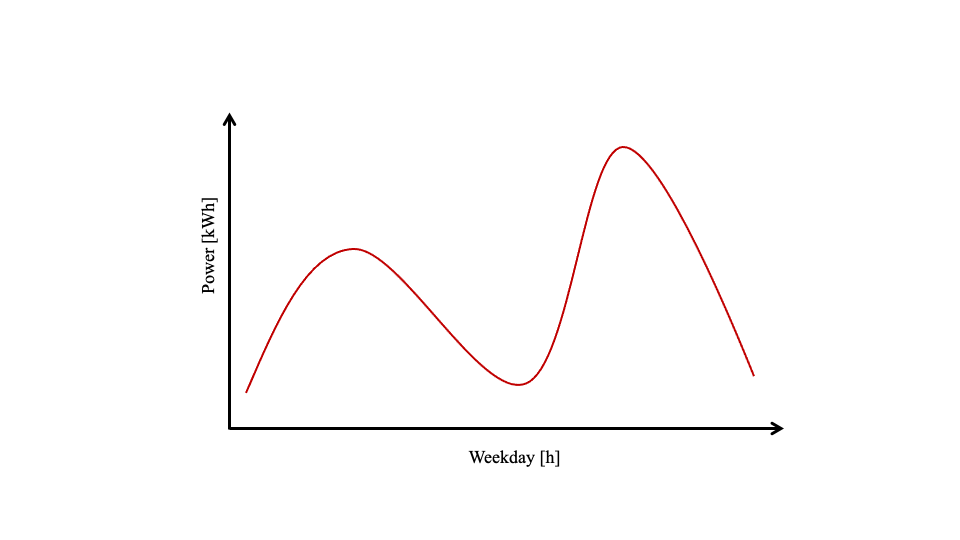
\includegraphics[width=0.9\textwidth]{Figures/profile_sketches/Slide1.png}
	\label{fig:daily_power_profile}
\end{figure}

Some refrences include daily usage profiles as a histogram of activation at a point in a day, such as figure \ref{fig:daily_act_profile}.

\begin{figure}[H]
	\centering
	\caption{"Histogram of daily activations profile for an appliance or a building"}
	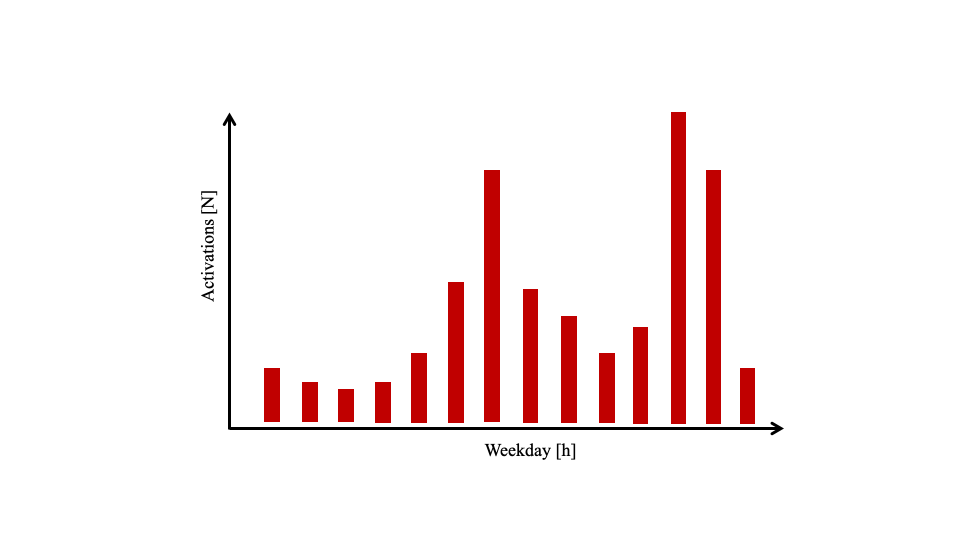
\includegraphics[width=0.9\textwidth]{Figures/profile_sketches/Slide5.png}
	\label{fig:daily_act_profile}
\end{figure}

All figures can present whole house usage or per device usage. Each representation has its pros and cons. 
To present more information sub-meter data can be used to represent whole house usage with per-appliance contributions.
Such as on figure \ref{fig:daily_act_m_profile} and \ref{fig:daily_power_m_profile}.

\begin{figure}[H]
	\centering
	\caption{"Histogram of daily activations profile for an appliance A and B"}
	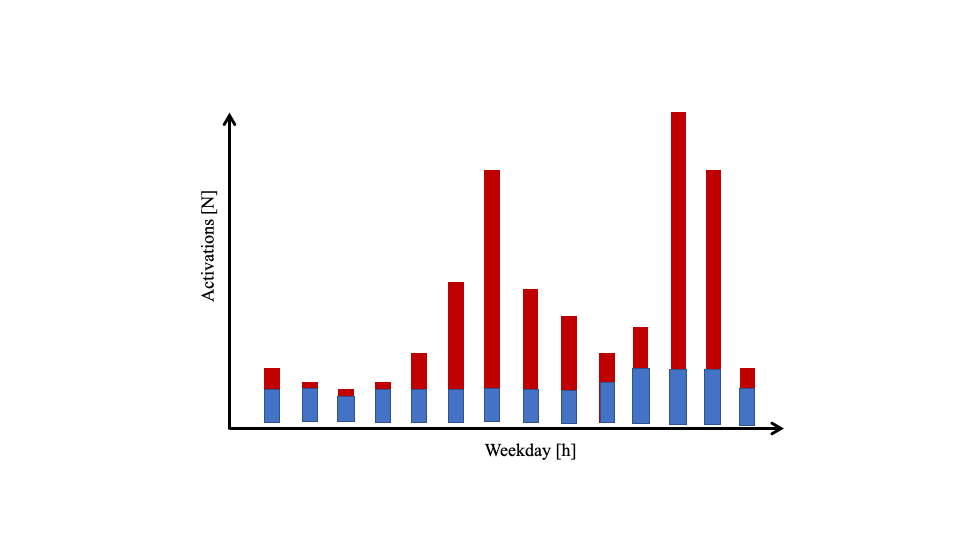
\includegraphics[width=0.9\textwidth]{Figures/profile_sketches/Slide8.png}
	\label{fig:daily_act_m_profile}
\end{figure}
\begin{figure}[H]
	\centering
	\caption{"Average weekday power consumption for appliances A, B and C"}
	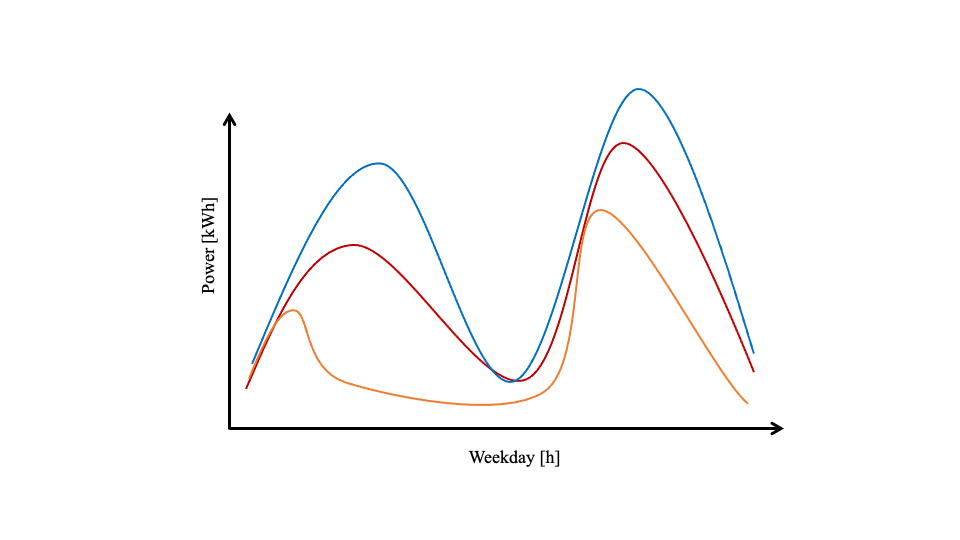
\includegraphics[width=0.9\textwidth]{Figures/profile_sketches/Slide2.png}
	\label{fig:daily_power_m_profile}
\end{figure}

To present as much information as possible all above-mentioned attributes 
can be presented in a multidimensional way such as heatmap in a way shown in figure \ref{fig:heatmap_2dtime} and \ref{fig:heatmap_all_appl}.

\begin{figure}[H]
	\centering
	\caption{"Number of daily activations / power consumption of one appliance / house in one month period"}
	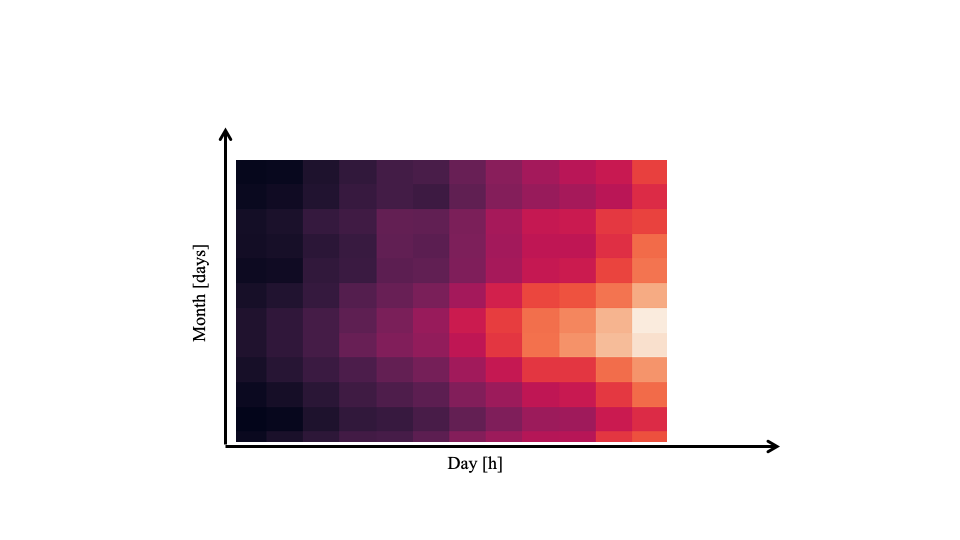
\includegraphics[width=0.9\textwidth]{Figures/profile_sketches/Slide10.png}
	\label{fig:heatmap_2dtime}
\end{figure}
\begin{figure}[H]
	\centering
	\caption{"Number of activations / power consumption for each appliance in one month period"}
	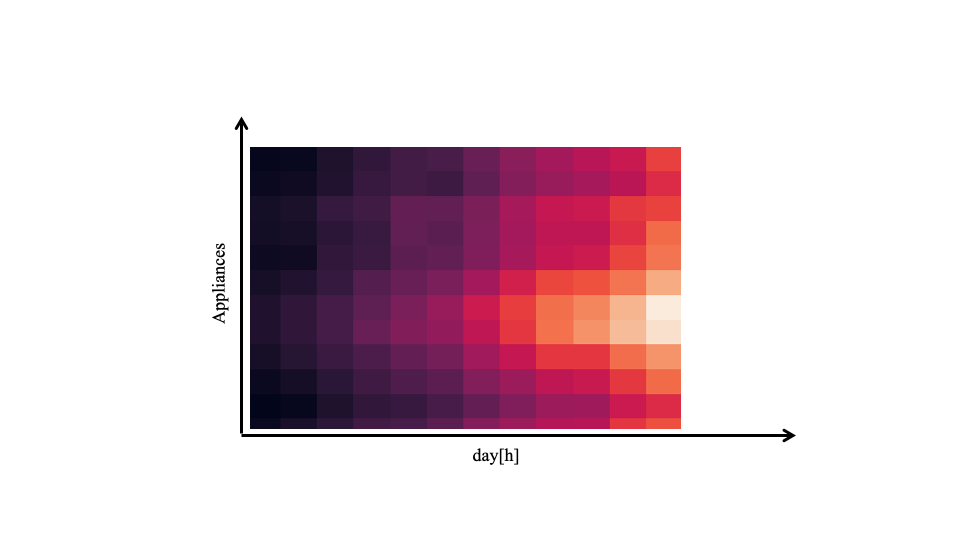
\includegraphics[width=0.9\textwidth]{Figures/profile_sketches/Slide12.png}
	\label{fig:heatmap_all_appl}
\end{figure}

Above shown profiles can be presented in combinations with each other, yielding a new way of presenting the data.
Bellow a map with combinations of above-mentioned profiles is presented. Some combinations that had similar output were grouped,
and some that were not logical were removed.  

\begin{figure}[H]
	\centering
	\caption{"Table of combinations"}
	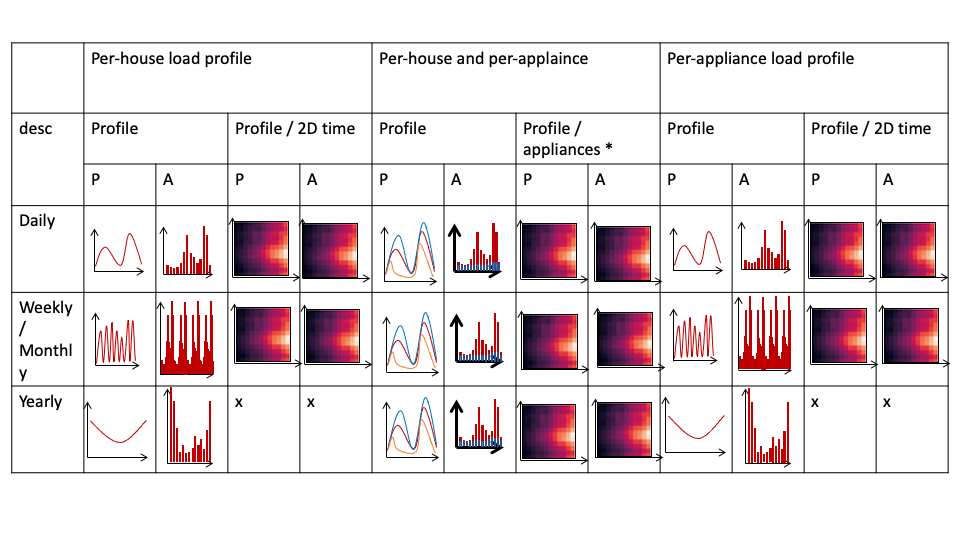
\includegraphics[width=0.9\textwidth]{Figures/profile_sketches/Slide14.png}
	\label{fig:map_fig}
\end{figure}

As can be seen from table \ref{tab:contributions}, most work (14 publications) has been done with standard daily load with
hole house power usage such as figure \ref{fig:daily_power_profile}. 
Quite a lot of work (6 publications) has been done with per appliance power profiles.
A few publications were based on weekly and yearly load profiles,
a few used two-dimensional time and power presentation and again others used diagregated data.
Only one publication found used activation and time based histogram such as 
shown on figure \ref{fig:daily_act_profile}. During the research I focused on publications
from minority classes, meaning not all existing publications for SLP are included. 
The purpose of table \ref{tab:contributions} is to present missing scientific contributions 
and publications pattern.  

\begin{table}[H]
	\caption{Table presents previously mentioned load profiles}
	\label{tab:contributions}

	\begin{tabular}{|l|cccc|cccc|cccc|}
	\hline
	Description                                                   & \multicolumn{4}{c|}{Per-house}                                                                                               & \multicolumn{4}{c|}{Per-appliance}                                                                                           & \multicolumn{4}{c|}{\begin{tabular}[c]{@{}c@{}}Per-house\\ per-appliance\end{tabular}}                                                         \\
																 & \multicolumn{2}{c|}{LP}                         & \multicolumn{2}{c|}{\begin{tabular}[c]{@{}c@{}}2D \\ time LP\end{tabular}} & \multicolumn{2}{c|}{LP}                         & \multicolumn{2}{c|}{\begin{tabular}[c]{@{}c@{}}2D\\  time LP\end{tabular}} & \multicolumn{2}{c|}{LP}                               & \multicolumn{2}{c|}{\begin{tabular}[c]{@{}c@{}}Appliances\\ side by side\end{tabular}} \\ \cline{1-1}
	\begin{tabular}[c]{@{}l@{}}Range of time\\ axis\end{tabular} & \multicolumn{1}{c|}{P} & \multicolumn{1}{c|}{A} & \multicolumn{1}{c|}{P}                         & A                         & \multicolumn{1}{c|}{P} & \multicolumn{1}{c|}{A} & \multicolumn{1}{c|}{P}                         & A                         & \multicolumn{1}{c|}{P}    & \multicolumn{1}{c|}{A}    & \multicolumn{1}{c|}{P}                               & A                               \\ \hline
	Daily                                                        & \multicolumn{1}{c|}{\begin{tabular}[c]{@{}c@{}} \citeyear*{Chuan2014} \\ \citeyear*{Csoknyai2019} \\ \citeyear*{H0} \\ \citeyear*{KAVOUSIAN2013184} \\ \citeyear*{CAPASSO1994} \\ \citeyear*{WALKER1985} \\ \citeyear*{GERBEC2005} \\ \citeyear*{Gao2018} \\ \citeyear*{Jeong2021} \\ \citeyear*{Joana2012} \\ \citeyear*{DER_heatmap_profile} \end{tabular}}  & \multicolumn{1}{c|}{}  & \multicolumn{1}{c|}{\begin{tabular}[c]{@{}l@{}} \citeyear*{2D_year_day_LP} \\ \citeyear*{Park2019} \\ \citeyear*{DER_heatmap_profile} \end{tabular}}   &    & \multicolumn{1}{c|}{\begin{tabular}[c]{@{}l@{}} \citeyear*{NILMAD2019} \\ \citeyear*{NILMAD22019} \\ \citeyear*{Issi2018} \\ \citeyear*{NILMAD2021} \\ \citeyear*{Castangia2021} \\ \citeyear*{occupancy2013}	\end{tabular}}  & \multicolumn{1}{c|}{\citeyear*{UKDALE}}  & \multicolumn{1}{c|}{}   &  \multicolumn{1}{c|}{}   & \multicolumn{1}{c|}{\begin{tabular}[c]{@{}l@{}} \citeyear*{Chuan2014} \\ \citeyear*{CAPASSO1994} \\ \citeyear*{Gao2018} 	\end{tabular}}   & \multicolumn{1}{c|}{}     & \multicolumn{1}{c|}{}      &    \\ \hline
	\begin{tabular}[c]{@{}l@{}}Weekly/\\ Monthly\end{tabular}    & \multicolumn{1}{c|}{\begin{tabular}[c]{@{}c@{}} \citeyear*{Csoknyai2019} \\ \citeyear*{H0} \\ \citeyear*{KAVOUSIAN2013184} \end{tabular}}  & \multicolumn{1}{c|}{}  & \multicolumn{1}{c|}{}                          &                           & \multicolumn{1}{c|}{}  & \multicolumn{1}{c|}{}  & \multicolumn{1}{c|}{}                          &                           & \multicolumn{1}{c|}{\citeyear*{weekly_per_appliance_LP}}    & \multicolumn{1}{c|}{}     & \multicolumn{1}{c|}{}                                &                                 \\ \hline
	Yearly                                                       & \multicolumn{1}{c|}{\begin{tabular}[c]{@{}c@{}} \citeyear*{Csoknyai2019} \\ \citeyear*{H0} \\ \citeyear*{KAVOUSIAN2013184} \end{tabular}}  & \multicolumn{1}{c|}{}  & \multicolumn{1}{c|}{}                          &                           & \multicolumn{1}{c|}{}  & \multicolumn{1}{c|}{}  & \multicolumn{1}{c|}{}                          &                           & \multicolumn{1}{c|}{}     & \multicolumn{1}{c|}{}     & \multicolumn{1}{c|}{}                                &                                 \\ \hline
	\end{tabular}
\end{table}

Table \ref{tab:use_cases} includes arranged publications from chapter \ref{Chapter5}. 
Similar pattern emerged as in table \ref{tab:contributions}. 

\begin{table}[H]
	\caption{Table presents refrences mentioned in use cases chapter}
	\label{tab:use_cases}
	\begin{tabular}{|l|cccc|cccc|cccc|}
	\hline
	Description &
	  \multicolumn{4}{c|}{Per-house} &
	  \multicolumn{4}{c|}{Per-appliance} &
	  \multicolumn{4}{c|}{\begin{tabular}[c]{@{}c@{}}Per-house\\ per-appliance\end{tabular}} \\
	 &
	  \multicolumn{2}{c|}{LP} &
	  \multicolumn{2}{c|}{\begin{tabular}[c]{@{}c@{}}2D \\ time LP\end{tabular}} &
	  \multicolumn{2}{c|}{LP} &
	  \multicolumn{2}{c|}{\begin{tabular}[c]{@{}c@{}}2D\\  time LP\end{tabular}} &
	  \multicolumn{2}{c|}{LP} &
	  \multicolumn{2}{c|}{\begin{tabular}[c]{@{}c@{}}Appliances\\ side by side\end{tabular}} \\ \cline{1-1}
	\begin{tabular}[c]{@{}l@{}}Range of time\\ axis\end{tabular} &
	  \multicolumn{1}{c|}{P} &
	  \multicolumn{1}{c|}{A} &
	  \multicolumn{1}{c|}{P} &
	  A &
	  \multicolumn{1}{c|}{P} &
	  \multicolumn{1}{c|}{A} &
	  \multicolumn{1}{c|}{P} &
	  A &
	  \multicolumn{1}{c|}{P} &
	  \multicolumn{1}{c|}{A} &
	  \multicolumn{1}{c|}{P} &
	  A \\ \hline
	Daily &
	  \multicolumn{1}{c|}{\begin{tabular}[c]{@{}c@{}} \citeyear*{energy_saving1} \\ \citeyear*{energy_saving3} \\ \citeyear*{EV2020} \\ \citeyear*{energyStealing2018} \\ \citeyear*{shift2015} \\ \citeyear*{optimiseCostShift2015} \\ \citeyear*{controll2014} \end{tabular}} &
	  \multicolumn{1}{c|}{} &
	  \multicolumn{1}{c|}{} &
	   &
	  \multicolumn{1}{c|}{\begin{tabular}[c]{@{}c@{}} \citeyear*{EV2020} \\ \citeyear*{elder1} \\ \citeyear*{elder2} \\   \citeyear*{occupancy2013}	  \end{tabular}} &
	  \multicolumn{1}{c|}{} &
	  \multicolumn{1}{c|}{} &
	   &
	  \multicolumn{1}{c|}{\citeyear*{Chuan2014}	 } &
	  \multicolumn{1}{c|}{} &
	  \multicolumn{1}{c|}{} &
	   \\ \hline
	\begin{tabular}[c]{@{}l@{}}Weekly/\\ Monthly\end{tabular} &
	  \multicolumn{1}{c|}{\begin{tabular}[c]{@{}c@{}} \citeyear*{energy_saving3} \\ \citeyear*{KAVOUSIAN2013184}  \end{tabular}} &
	  \multicolumn{1}{c|}{} &
	  \multicolumn{1}{c|}{} &
	   &
	  \multicolumn{1}{c|}{} &
	  \multicolumn{1}{c|}{} &
	  \multicolumn{1}{c|}{} &
	   &
	  \multicolumn{1}{c|}{} &
	  \multicolumn{1}{c|}{} &
	  \multicolumn{1}{c|}{} &
	   \\ \hline
	Yearly &
	  \multicolumn{1}{c|}{\begin{tabular}[c]{@{}c@{}}\citeyear*{energy_saving3}\end{tabular}} &
	  \multicolumn{1}{c|}{} &
	  \multicolumn{1}{c|}{} &
	   &
	  \multicolumn{1}{c|}{} &
	  \multicolumn{1}{c|}{} &
	  \multicolumn{1}{c|}{} &
	   &
	  \multicolumn{1}{c|}{} &
	  \multicolumn{1}{c|}{} &
	  \multicolumn{1}{c|}{} &
	   \\ \hline
	\end{tabular}
\end{table}

Table \ref{tab:groups} presents same publications as \ref{tab:use_cases},
but only group names are shown. Table clearly indicates how groups are arranged.
Where anomaly detection and eldery care are domanating in per appliance starnard load profile,
energy saving and grid management are dimainatin in per-house sub group. 

\begin{table}[H]
    \caption{Table presents refrences mentioned in use cases chapter}
	\label{tab:groups}
    \begin{adjustbox}{width=1.2\textwidth,center=\textwidth} 
        \begin{tabular}{|l|cccc|cccc|cccc|}
            \hline
            \begin{tabular}[c]{@{}l@{}}ES - energy saving\\ GM - grid managment\\ AD - anomaly detection\\ EC - eldery care\\ X - unfeasable\end{tabular} &
              \multicolumn{4}{c|}{Per-house} &
              \multicolumn{4}{c|}{Per-appliance} &
              \multicolumn{4}{c|}{\begin{tabular}[c]{@{}c@{}}Per-house\\ per-appliance\end{tabular}} \\ \cline{2-13} 
             &
              \multicolumn{2}{c|}{LP} &
              \multicolumn{2}{c|}{\begin{tabular}[c]{@{}c@{}}2D \\ time LP\end{tabular}} &
              \multicolumn{2}{c|}{LP} &
              \multicolumn{2}{c|}{\begin{tabular}[c]{@{}c@{}}2D\\  time LP\end{tabular}} &
              \multicolumn{2}{c|}{LP} &
              \multicolumn{2}{c|}{\begin{tabular}[c]{@{}c@{}}Appliances\\ side by side\end{tabular}} \\ \hline
            \begin{tabular}[c]{@{}l@{}}Range of time\\ axis\end{tabular} &
              \multicolumn{1}{c|}{P} &
              \multicolumn{1}{c|}{A} &
              \multicolumn{1}{c|}{P} &
              A &
              \multicolumn{1}{c|}{P} &
              \multicolumn{1}{c|}{A} &
              \multicolumn{1}{c|}{P} &
              A &
              \multicolumn{1}{c|}{P} &
              \multicolumn{1}{c|}{A} &
              \multicolumn{1}{c|}{P} &
              A \\ \hline
            Daily &
              \multicolumn{1}{c|}{ES,GM} &
              \multicolumn{1}{c|}{} &
              \multicolumn{1}{c|}{} &
               &
              \multicolumn{1}{c|}{\begin{tabular}[c]{@{}c@{}}AD,EC,\\ ES\end{tabular}} &
              \multicolumn{1}{c|}{} &
              \multicolumn{1}{c|}{} &
               &
              \multicolumn{1}{c|}{GM} &
              \multicolumn{1}{c|}{} &
              \multicolumn{1}{c|}{} &
               \\ \hline
            \begin{tabular}[c]{@{}l@{}}Weekly/\\ Monthly\end{tabular} &
              \multicolumn{1}{c|}{ES} &
              \multicolumn{1}{c|}{} &
              \multicolumn{1}{c|}{} &
               &
              \multicolumn{1}{c|}{} &
              \multicolumn{1}{c|}{} &
              \multicolumn{1}{c|}{} &
               &
              \multicolumn{1}{c|}{} &
              \multicolumn{1}{c|}{} &
              \multicolumn{1}{c|}{} &
               \\ \hline
            Yearly &
              \multicolumn{1}{c|}{ES} &
              \multicolumn{1}{c|}{} &
              \multicolumn{1}{c|}{X} &
              X &
              \multicolumn{1}{c|}{} &
              \multicolumn{1}{c|}{} &
              \multicolumn{1}{c|}{X} &
              X &
              \multicolumn{1}{c|}{} &
              \multicolumn{1}{c|}{} &
              \multicolumn{1}{c|}{} &
               \\ \hline
            \end{tabular}
    \end{adjustbox} 
    \end{table}

Figures listed above clearly depict the void not filled by publications. 
All through there are blank spaces, they still have a possible 
use case. 
In table \ref{tab:groups_proposed} spaces are filled 
with possible use cases for given load profiles. 

\begin{table}[H]
    \caption{"Proposed use cases for profiles"}
    \label{tab:groups_proposed}
    \begin{adjustbox}{width=1.2\textwidth,center=\textwidth} 
    \begin{tabular}{|l|cccc|cccc|cccc|}
    \hline
    \begin{tabular}[c]{@{}l@{}}ES - energy saving\\ GM - grid managment\\ AD - anomaly detection\\ EC - eldery care\\ X - unfeasable\end{tabular} &
      \multicolumn{4}{c|}{Per-house} &
      \multicolumn{4}{c|}{Per-appliance} &
      \multicolumn{4}{c|}{\begin{tabular}[c]{@{}c@{}}Per-house\\ per-appliance\end{tabular}} \\ \cline{2-13} 
     &
      \multicolumn{2}{c|}{LP} &
      \multicolumn{2}{c|}{\begin{tabular}[c]{@{}c@{}}2D \\ time LP\end{tabular}} &
      \multicolumn{2}{c|}{LP} &
      \multicolumn{2}{c|}{\begin{tabular}[c]{@{}c@{}}2D\\  time LP\end{tabular}} &
      \multicolumn{2}{c|}{LP} &
      \multicolumn{2}{c|}{\begin{tabular}[c]{@{}c@{}}Appliances\\ side by side\end{tabular}} \\ \hline
    \begin{tabular}[c]{@{}l@{}}Range of time\\ axis\end{tabular} &
      \multicolumn{1}{c|}{P} &
      \multicolumn{1}{c|}{A} &
      \multicolumn{1}{c|}{P} &
      A &
      \multicolumn{1}{c|}{P} &
      \multicolumn{1}{c|}{A} &
      \multicolumn{1}{c|}{P} &
      A &
      \multicolumn{1}{c|}{P} &
      \multicolumn{1}{c|}{A} &
      \multicolumn{1}{c|}{P} &
      A \\ \hline
    Daily &
      \multicolumn{1}{c|}{\begin{tabular}[c]{@{}c@{}}AD,\\ ES,GM,\end{tabular}} &
      \multicolumn{1}{c|}{\begin{tabular}[c]{@{}c@{}}AD,\\ ES,GM,\end{tabular}} &
      \multicolumn{1}{c|}{ES,GM} &
      ES,GM &
      \multicolumn{1}{c|}{\begin{tabular}[c]{@{}c@{}}AD,EC,\\ ES,GM\end{tabular}} &
      \multicolumn{1}{c|}{\begin{tabular}[c]{@{}c@{}}AD,EC,\\ ES,GM\end{tabular}} &
      \multicolumn{1}{c|}{\begin{tabular}[c]{@{}c@{}}AD,EC,\\ ES,GM\end{tabular}} &
      \begin{tabular}[c]{@{}c@{}}AD,EC,\\ ES,GM\end{tabular} &
      \multicolumn{1}{c|}{\begin{tabular}[c]{@{}c@{}}AD,EC,\\ ES,GM\end{tabular}} &
      \multicolumn{1}{c|}{\begin{tabular}[c]{@{}c@{}}AD,EC,\\ ES,GM\end{tabular}} &
      \multicolumn{1}{c|}{\begin{tabular}[c]{@{}c@{}}AD,EC,\\ ES,GM\end{tabular}} &
      \begin{tabular}[c]{@{}c@{}}AD,EC,\\ ES,GM\end{tabular} \\ \hline
    \begin{tabular}[c]{@{}l@{}}Weekly/\\ Monthly\end{tabular} &
      \multicolumn{1}{c|}{\begin{tabular}[c]{@{}c@{}}AD,\\ ES,GM\end{tabular}} &
      \multicolumn{1}{c|}{\begin{tabular}[c]{@{}c@{}}AD,\\ ES,GM,\end{tabular}} &
      \multicolumn{1}{c|}{ES,GM} &
      ES,GM &
      \multicolumn{1}{c|}{\begin{tabular}[c]{@{}c@{}}AD,\\ ES,GM\end{tabular}} &
      \multicolumn{1}{c|}{\begin{tabular}[c]{@{}c@{}}AD,\\ ES,GM\end{tabular}} &
      \multicolumn{1}{c|}{\begin{tabular}[c]{@{}c@{}}AD,\\ ES,GM\end{tabular}} &
      \begin{tabular}[c]{@{}c@{}}AD,\\ ES,GM\end{tabular} &
      \multicolumn{1}{c|}{\begin{tabular}[c]{@{}c@{}}AD,\\ ES,GM\end{tabular}} &
      \multicolumn{1}{c|}{\begin{tabular}[c]{@{}c@{}}AD,\\ ES,GM\end{tabular}} &
      \multicolumn{1}{c|}{\begin{tabular}[c]{@{}c@{}}AD,\\ ES,GM\end{tabular}} &
      \begin{tabular}[c]{@{}c@{}}AD,\\ ES,GM\end{tabular} \\ \hline
    Yearly &
      \multicolumn{1}{c|}{ES,GM} &
      \multicolumn{1}{c|}{ES,GM,} &
      \multicolumn{1}{c|}{X} &
      X &
      \multicolumn{1}{c|}{\begin{tabular}[c]{@{}c@{}}AD,\\ ES,GM\end{tabular}} &
      \multicolumn{1}{c|}{\begin{tabular}[c]{@{}c@{}}AD,\\ ES,GM\end{tabular}} &
      \multicolumn{1}{c|}{X} &
      X &
      \multicolumn{1}{c|}{} &
      \multicolumn{1}{c|}{\begin{tabular}[c]{@{}c@{}}AD,\\ ES,GM\end{tabular}} &
      \multicolumn{1}{c|}{\begin{tabular}[c]{@{}c@{}}AD,\\ ES,GM\end{tabular}} &
      \begin{tabular}[c]{@{}c@{}}AD,\\ ES,GM\end{tabular} \\ \hline
    \end{tabular}
    \end{adjustbox}
\end{table}


It is true that some combinations are illogical and others are less useful in 
practical sense. Next table will try to rate profiles 
based on two main features. 
First is how data is presented to the user,
meaning that load profile is clear at what it is presenting.
Second is the efectivness when being used in an algoritm.
These parameters cannot be measured, it is possible
to extrapolate the publications pattern, to find 
usefull gaps. If we assume that larger the number of publications
and larger the number of use cases the higher the utility rate of a profile,
we can spot a pattern. 
Using this pattern we propose a following table. table has four possible classes. 

\begin{outline}
\1 1 - Load profile has a high utility rate and has high research potential. 
\1 2 - Load profiles does not satisfy one of above-mentioned features and has mid research potential
\1 3 - Load profile does not suffice none of the above-mentioned features and has low research potential
\1 X - Load profile does not make any sense and cannot be generated. 
\end{outline}

\begin{table}[H]
    \caption{Proposed classification of profiles}
    \label{tab:classified_profiles}
    \begin{tabular}{|l|cccc|cccc|cccc|}
    \hline
     &
      \multicolumn{4}{c|}{Per-house} &
      \multicolumn{4}{c|}{Per-appliance} &
      \multicolumn{4}{c|}{\begin{tabular}[c]{@{}c@{}}Per-house\\ per-appliance\end{tabular}} \\ \cline{2-13} 
     &
      \multicolumn{2}{c|}{LP} &
      \multicolumn{2}{c|}{\begin{tabular}[c]{@{}c@{}}2D \\ time LP\end{tabular}} &
      \multicolumn{2}{c|}{LP} &
      \multicolumn{2}{c|}{\begin{tabular}[c]{@{}c@{}}2D\\  time LP\end{tabular}} &
      \multicolumn{2}{c|}{LP} &
      \multicolumn{2}{c|}{\begin{tabular}[c]{@{}c@{}}Appliances\\ side by side\end{tabular}} \\ \hline
    \begin{tabular}[c]{@{}l@{}}Range of time\\ axis\end{tabular} &
      \multicolumn{1}{c|}{P} &
      \multicolumn{1}{c|}{A} &
      \multicolumn{1}{c|}{P} &
      A &
      \multicolumn{1}{c|}{P} &
      \multicolumn{1}{c|}{A} &
      \multicolumn{1}{c|}{P} &
      A &
      \multicolumn{1}{c|}{P} &
      \multicolumn{1}{c|}{A} &
      \multicolumn{1}{c|}{P} &
      A \\ \hline
    Daily &
      \multicolumn{1}{c|}{1} &
      \multicolumn{1}{c|}{2} &
      \multicolumn{1}{c|}{1} &
      1 &
      \multicolumn{1}{c|}{1} &
      \multicolumn{1}{c|}{1} &
      \multicolumn{1}{c|}{1} &
      1 &
      \multicolumn{1}{c|}{1} &
      \multicolumn{1}{c|}{1} &
      \multicolumn{1}{c|}{1} &
      1 \\ \hline
    \begin{tabular}[c]{@{}l@{}}Weekly/\\ Monthly\end{tabular} &
      \multicolumn{1}{c|}{1} &
      \multicolumn{1}{c|}{2} &
      \multicolumn{1}{c|}{3} &
      3 &
      \multicolumn{1}{c|}{1} &
      \multicolumn{1}{c|}{1} &
      \multicolumn{1}{c|}{3} &
      3 &
      \multicolumn{1}{c|}{2} &
      \multicolumn{1}{c|}{2} &
      \multicolumn{1}{c|}{2} &
      2 \\ \hline
    Yearly &
      \multicolumn{1}{c|}{1} &
      \multicolumn{1}{c|}{3} &
      \multicolumn{1}{c|}{X} &
      X &
      \multicolumn{1}{c|}{2} &
      \multicolumn{1}{c|}{2} &
      \multicolumn{1}{c|}{X} &
      X &
      \multicolumn{1}{c|}{3} &
      \multicolumn{1}{c|}{3} &
      \multicolumn{1}{c|}{2} &
      2 \\ \hline
    \end{tabular}
\end{table}

Using all above mentioned tables we can use superpoistion
to generate a universal table, that will present possible 
researh directions. 
Table has to satisfy following rules. 
First is that load profile should have no publications
or yet discovered use cases. Second one is that 
load profile should be at least in second class. 

\begin{table}[H]
    \caption{Possible future research contributions}
    \label{tab:future_rd}
    \begin{tabular}{|l|cccc|cccc|cccc|}
    \hline
     &
      \multicolumn{4}{c|}{Per-house} &
      \multicolumn{4}{c|}{Per-appliance} &
      \multicolumn{4}{c|}{\begin{tabular}[c]{@{}c@{}}Per-house\\ per-appliance\end{tabular}} \\ \cline{2-13} 
     &
      \multicolumn{2}{c|}{LP} &
      \multicolumn{2}{c|}{\begin{tabular}[c]{@{}c@{}}2D \\ time LP\end{tabular}} &
      \multicolumn{2}{c|}{LP} &
      \multicolumn{2}{c|}{\begin{tabular}[c]{@{}c@{}}2D\\  time LP\end{tabular}} &
      \multicolumn{2}{c|}{LP} &
      \multicolumn{2}{c|}{\begin{tabular}[c]{@{}c@{}}Appliances\\ side by side\end{tabular}} \\ \hline
    \begin{tabular}[c]{@{}l@{}}Range of time\\ axis\end{tabular} &
      \multicolumn{1}{c|}{P} &
      \multicolumn{1}{c|}{A} &
      \multicolumn{1}{c|}{P} &
      A &
      \multicolumn{1}{c|}{P} &
      \multicolumn{1}{c|}{A} &
      \multicolumn{1}{c|}{P} &
      A &
      \multicolumn{1}{c|}{P} &
      \multicolumn{1}{c|}{A} &
      \multicolumn{1}{c|}{P} &
      A \\ \hline
    Daily &
      \multicolumn{1}{c|}{} &
      \multicolumn{1}{c|}{2} &
      \multicolumn{1}{c|}{} &
      1 &
      \multicolumn{1}{c|}{} &
      \multicolumn{1}{c|}{} &
      \multicolumn{1}{c|}{1} &
      1 &
      \multicolumn{1}{c|}{} &
      \multicolumn{1}{c|}{1} &
      \multicolumn{1}{c|}{1} &
      1 \\ \hline
    \begin{tabular}[c]{@{}l@{}}Weekly/\\ Monthly\end{tabular} &
      \multicolumn{1}{c|}{} &
      \multicolumn{1}{c|}{2} &
      \multicolumn{1}{c|}{} &
       &
      \multicolumn{1}{c|}{1} &
      \multicolumn{1}{c|}{1} &
      \multicolumn{1}{c|}{} &
       &
      \multicolumn{1}{c|}{} &
      \multicolumn{1}{c|}{} &
      \multicolumn{1}{c|}{2} &
      2 \\ \hline
    Yearly &
      \multicolumn{1}{c|}{} &
      \multicolumn{1}{c|}{} &
      \multicolumn{1}{c|}{} &
       &
      \multicolumn{1}{c|}{2} &
      \multicolumn{1}{c|}{2} &
      \multicolumn{1}{c|}{} &
       &
      \multicolumn{1}{c|}{} &
      \multicolumn{1}{c|}{} &
      \multicolumn{1}{c|}{2} &
      2 \\ \hline
    \end{tabular}
\end{table}

Table \ref{tab:future_rd} presents load profiles that we will pursue in 
this paper. We will focus on profiles from the first class and activation
frequency type of usage. When aforementioned parameters are applied, 
the obtained results is table \ref{tab:our_rd}

\begin{table}[H]
    \caption{Load profiles to be pursued }
    \label{tab:our_rd}
    \begin{tabular}{|l|cccc|cccc|cccc|}
    \hline
     &
      \multicolumn{4}{c|}{Per-house} &
      \multicolumn{4}{c|}{Per-appliance} &
      \multicolumn{4}{c|}{\begin{tabular}[c]{@{}c@{}}Per-house\\ per-appliance\end{tabular}} \\ \cline{2-13} 
     &
      \multicolumn{2}{c|}{LP} &
      \multicolumn{2}{c|}{\begin{tabular}[c]{@{}c@{}}2D \\ time LP\end{tabular}} &
      \multicolumn{2}{c|}{LP} &
      \multicolumn{2}{c|}{\begin{tabular}[c]{@{}c@{}}2D\\  time LP\end{tabular}} &
      \multicolumn{2}{c|}{LP} &
      \multicolumn{2}{c|}{\begin{tabular}[c]{@{}c@{}}Appliances\\ side by side\end{tabular}} \\ \hline
    \begin{tabular}[c]{@{}l@{}}Range of time\\ axis\end{tabular} &
      \multicolumn{1}{c|}{P} &
      \multicolumn{1}{c|}{A} &
      \multicolumn{1}{c|}{P} &
      A &
      \multicolumn{1}{c|}{P} &
      \multicolumn{1}{c|}{A} &
      \multicolumn{1}{c|}{P} &
      A &
      \multicolumn{1}{c|}{P} &
      \multicolumn{1}{c|}{A} &
      \multicolumn{1}{c|}{P} &
      A \\ \hline
    Daily &
      \multicolumn{1}{c|}{} &
      \multicolumn{1}{c|}{} &
      \multicolumn{1}{c|}{} &
      1 &
      \multicolumn{1}{c|}{} &
      \multicolumn{1}{c|}{} &
      \multicolumn{1}{c|}{} &
      1 &
      \multicolumn{1}{c|}{} &
      \multicolumn{1}{c|}{1} &
      \multicolumn{1}{c|}{} &
      1 \\ \hline
    \begin{tabular}[c]{@{}l@{}}Weekly/\\ Monthly\end{tabular} &
      \multicolumn{1}{c|}{} &
      \multicolumn{1}{c|}{} &
      \multicolumn{1}{c|}{} &
       &
      \multicolumn{1}{c|}{} &
      \multicolumn{1}{c|}{1} &
      \multicolumn{1}{c|}{} &
       &
      \multicolumn{1}{c|}{} &
      \multicolumn{1}{c|}{} &
      \multicolumn{1}{c|}{} &
       \\ \hline
    Yearly &
      \multicolumn{1}{c|}{} &
      \multicolumn{1}{c|}{} &
      \multicolumn{1}{c|}{} &
       &
      \multicolumn{1}{c|}{} &
      \multicolumn{1}{c|}{} &
      \multicolumn{1}{c|}{} &
       &
      \multicolumn{1}{c|}{} &
      \multicolumn{1}{c|}{} &
      \multicolumn{1}{c|}{} &
       \\ \hline
    \end{tabular}
    \end{table}






